% !TEX root = ./paper.tex
% Design note to remember to explain: multi-stream \tcpls must increase the lower
% 64 bits of the IV to keep using a counter starting a 0. (though, we need a
% limit on the number of paralel stream creation)

\begin{figure}[!t]
  \begin{center}
      \vspace{-1.5cm}
    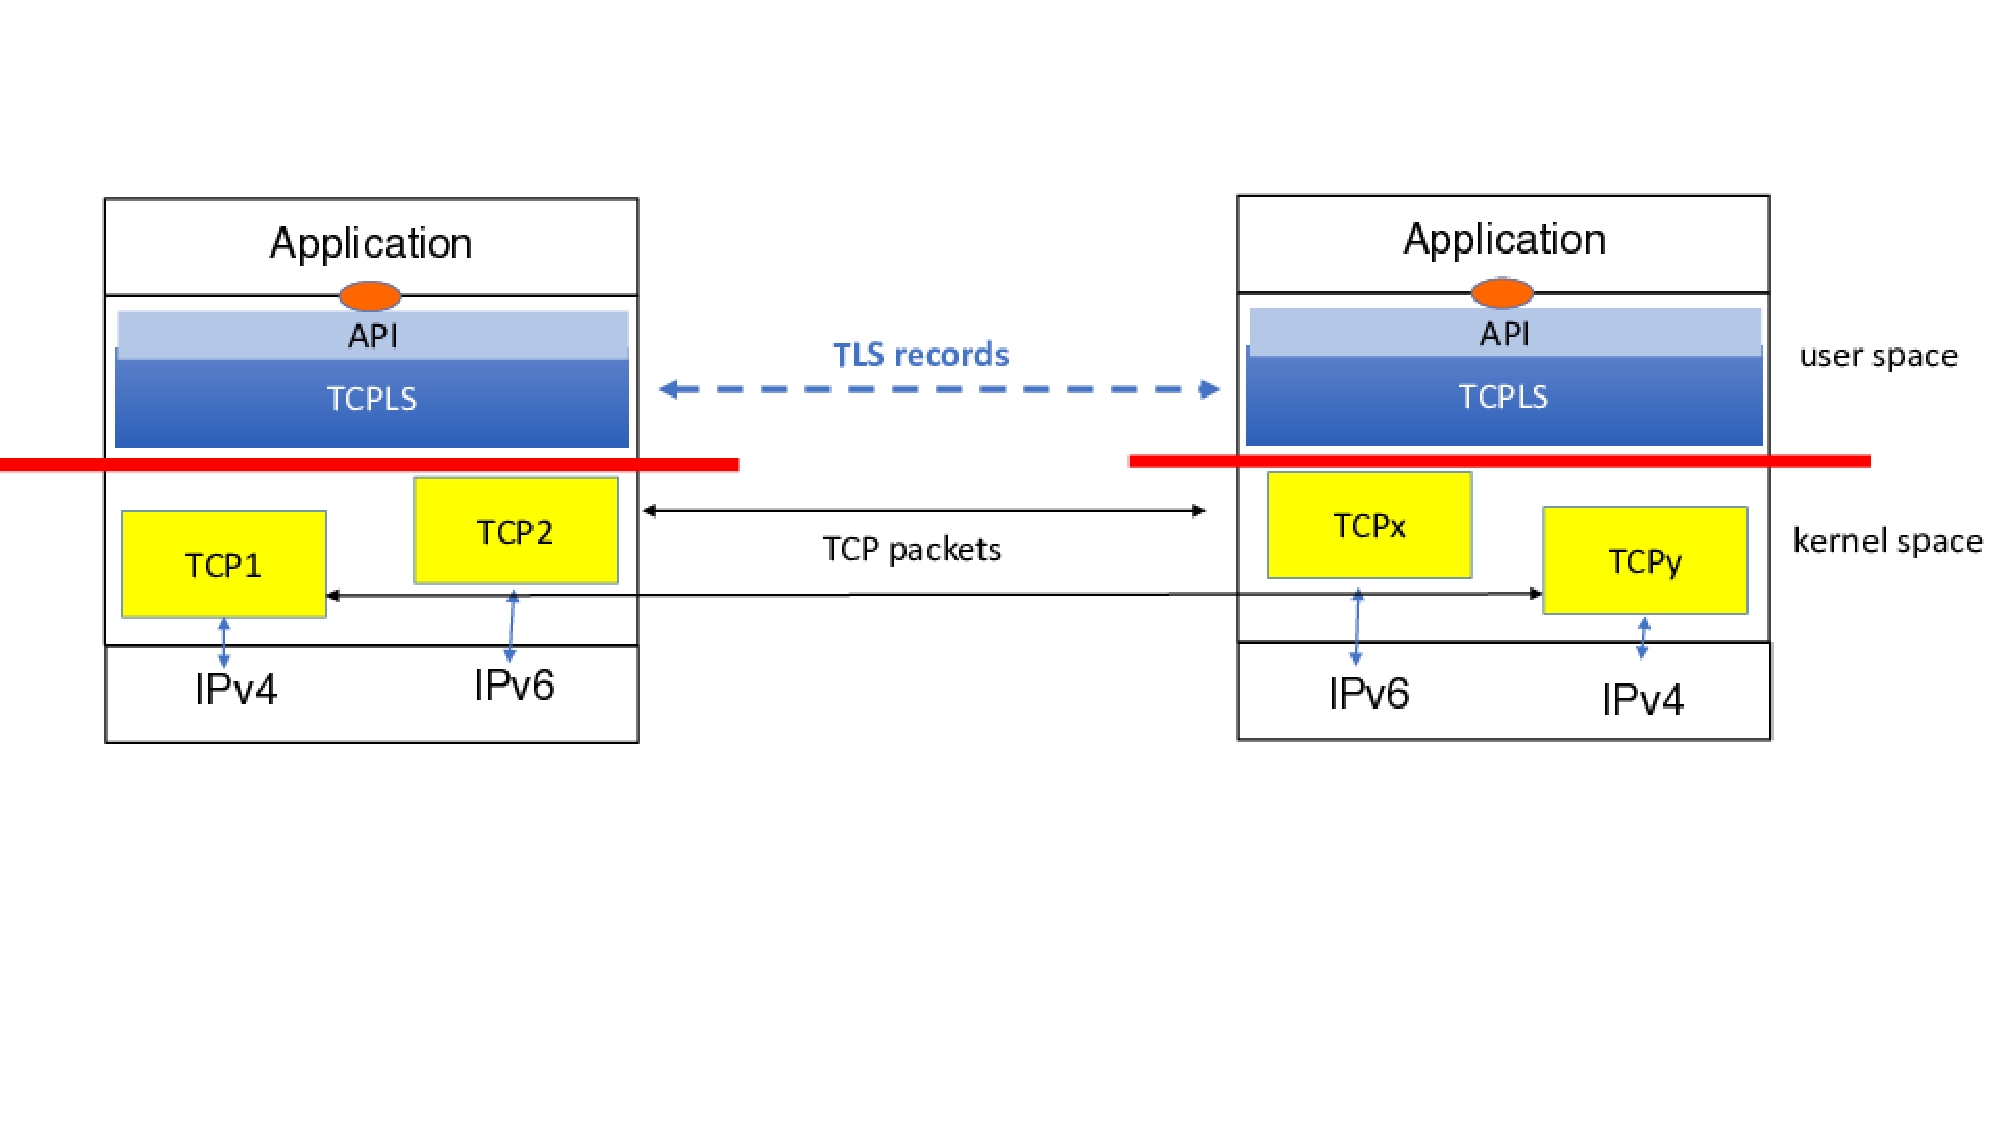
\includegraphics[width=8cm]{figures/tcpls-fig2.pdf}
  \end{center}
  \vspace{-1.5cm}
  \caption{TCPLS in the stack.}
  \label{fig:arch}
    \vspace{-0.5cm}
\end{figure}



\subsection{The Secure Control Channel}\label{sec:extending}

\tls 1.3~\cite{rfc8446} has been designed with careful consideration for
potential extensions. It supports the \textsc{EncryptedExtensions} message sent
by the server alongside the \textsc{ServerHello}. Any extension sent with the
\textsc{ServerHello} message is encrypted with the handshake key, and is not
part of the context used to derive the eventual application key.
%Such a design choice eases dealing with implementations
%not supporting a particular option since an opportunistic transmission
%of an option will not affect the handshake outcome.

A reasonable approach to designing extensibility mechanisms in today's Internet
is to avoid leaking any information that could help an on-path attacker
recognize specific users or applications. Indeed, censorship~\cite{Morshed2017a,
  Gosain2017a,Chai2019a} can be easily implemented when protocol messages can be
distinguished, and avoiding trivial opportunities to implement censorship should
become the bare minimum in designing a new protocol. \tcpls's control protocol
considers those problems by avoiding unencrypted data within the
\textsc{ClientHello}.

In our design, the client indicates its willingness to use \tcpls with a
transport parameter in the \textsc{ClientHello}. Upon reception of this
parameter, the server can opportunistically send lightweight \tcpls data and
\tcp options as \textsc{EncryptedExtensions}. If the client does not support
some extension, it echoes back an alert with the value of the option it does not
recognize, but the connection continues.

The server or the client can also send \tcpls control messages after the
handshake. These control messages take advantage of the \tls 1.3 content-type
extensibility feature to avoid middlebox interference. Indeed, in \tls 1.3, the
Record Protocol ensures that any new message appears as an \textsc{AppData}
message type while the true content type (TType) is stored at the end of the
encrypted payload. As an example, Fig.~\ref{ex_record}
shows the \tcpls control message structure that carries the
\tcp User Timeout~\cite{rfc5482} option. $TType$ is the true type of this
record (TCP\_OPTION), while its Type is set to $APPDATA$.

% Discussing the lack of extensibility of TLS 1.3;
\begin{figure}
  \begin{bytefield}[bitwidth=0.47em]{40}
    \bitheader[lsb=0,bitformatting={\tiny\rotatebox[origin=B]{90}}]{0-39} \\
    \begin{rightwordgroup}{Header}
      \bitbox{8}{Type} & \bitbox{16}{Version} & \bitbox{16}{Length}
    \end{rightwordgroup}\\
    \begin{rightwordgroup}{Payload}
      \bitbox{16}{Option Type} & \bitbox{16}{User Timeout} & \bitbox{8}{TType}
     %&\wordbox[lrb]{1}{Padding... (to match the AEAD block size)}
    \end{rightwordgroup}\\
  \end{bytefield}
  \caption{A new type of \tls Record containing a \tcp option.}
  \label{ex_record}
\end{figure}



\subsection{Datastreams}
\label{sec:datastreams}

\paragraph*{Cryptographic Details and Tricks}
In \tcpls, each stream has its own cryptographic context. They use the same key
but derive the blockcipher IV (Initial Vector, also called cryptographic nonce)
such that nonce-misuse cannot happen while the record sequence number within
each stream starts at 0. Only one application-level key is used for $N$ streams,
for each direction.  The reason behind this design choice is to avoid security
degradation with the usage of multiple keys (by a factor $k$ with $k$
keys)~\cite{chatterjee2011another}. To understand the trick behind every
stream sequences to start at 0, we need some AEAD details. In \tcpls, the AEAD
nonce must be of unique use when encrypting and decrypting a message. The
initial nonce must also be unpredictable for an adversary observig the
handshake, and is in practice derived from the \tls handshake session secret in
a similar fashion than the \tls keys. The nonce size is specified to be from
$96$ bits to $128$ bits depending on the underlying cipher used. In all cases,
for a nonce of size $N$ in \tls, the cryptographic nonce given to the underlying
cipher is computed from concatenating the $N-64$ leftmost bits with the 64 lower
bits xored with the record's implicit sequence number encoded in 64 bits. The
lower 64 bits xoring gives more unpredictability to the nonce when the same
plaintext is encrypted multiple times with the same
key~\cite{bellare2016multi,hoang2018multi}. This design means that we give to
the underlaying cipher the 32 upper bits untouched. The resulting value is then
incremented at most 1024 times starting from the leftmost bits to encrypt a \tls
record of maximum size (16384 bytes, i.e, 1024 times 128 bits for the the
minimum block size). So, we observe that 7 bits among those 32 bits are
untouchable, leading to at least 25 bits to encode a unique stream number.
Encoding such a unique number in this space of the cryptographic nonce allows
each stream to start its sequence number at 0 while encrypting its record with
the same key. This observation means that we can create independant
cryptographic context based on a tweak of the cryptographic nonce, which allows
streams to encrypt and decrypt independently of each other, with the same key
value. This trick maintains AEAD's core assumption (uniqueness of nonce), which
means that the state of art AEAD's security proof starting from that assumption
applies to our design~\cite{chatterjee2011another} and guarantees the security
of our scheme.

\paragraph*{Multiple Streams over the Same Transport}
Having a separate cryptographic context means that \tcpls can do concurrent
encryption and decryption between streams while maintaining decryption
correctness and security, and potentially also use this capability to process
streams over multiple cores. Finally, if we have multiple streams over the same
\tcp connection, \tcpls does not explicitely know which received data belongs to
which stream. To obtain this information, we either require to modify the
associated information within \tls records to add a stream id (this associated
data is not encrypted but the AEAD cipher authenticates them). This choice
means potential middlebox interference, which we chose to avoid. The other
option is to leverage the AEAD cipher to check the authentication tag of the
incoming record until we find the stream that properly verifies the tag. This
operation is lightweight: it does not require full decryption of the record
because \tls 1.3 uses AEAD ciphers doing Encrypt then MAC (and MAC then
Decrypt), and looking for the right stream needs to be performed once each time
the application writes to another stream over the same \tcp connection.

Note that, security-wise, each failed decryption is considered as a
forgery attempt. However, we have large limits on the confidentiality and
integrity with all AEAD ciphers~\cite{luykx2015limits, aeadlimits} before a
successful forgery may be considered as a non-negligeable probability.

%Streams are an interesting abstraction for applications. Experience with HTTP/2
%has shown that head-of-line blocking was an important factor in web performance.
%This motivated the first QUIC design \cite{langley2017quic}. If all data streams
%are mapped on the same underlying \tcp connection, head-of-line blocking remains
%possible. However, this blocking can be prevented by using different \tcp
%connections to transport the different data streams.


\subsection{Multipath in a Modern Transport Protocol}
\label{sec:multipath}

\paragraph*{The \tcpls approach to Multipath}
\tcpls enables the client or the server to associate new \tcp connections to an
existing \tcpls connection. This is similar to what \mptcp
does~\cite{raiciu2012hard,rfc6824}, but with some differences. First, \mptcp
supports only one bytestream. Second, \tcpls does not suffer from the same
security limitations as \mptcp. To secure the attachment of additional subflows,
\mptcp hosts exchange keys in plaintext during the handshake~\cite{rfc6824,
  rfc8684}. These keys are then used later to authenticate the attachment of
subflows to a connection. An attacker that has observed the initial handshake
can attach any subflow to an existing \mptcp connection~\cite{rfc6181}.
Finally,  \tcpls offers
several mode of multipathing. An aggregation mode is an option to take advantage of
multiple network interfaces and safely splitting an applical-level object over
them. However, \tcpls also offers multiple paths without bandwidth aggregation.
This is a choice left to the application using the API, and it has several
advantages and inconvenients compared to the aggregation mode. For example, the
aggregation mode is simple to use and can potentially saturate all available
network paths but creates HOL blocking, since packets sent over different TCP
connections need to be eventually re-ordered. This mode is also more CPU
costly, since a zero-copy codepath is technically possible only when the packets
arrive in order. In the multipath non-aggregated mode, the application needs to
take care to fully send an application-level object over the same stream, since
the ordering is only guaranteed per-stream in this mode. However, \tcpls
guarantees this mode to offer zero-copy of the decrypted application data, which
makes this mode potentially quite interesting for application protocol such as
HTTP that needs to fetch multiple application objects at the same time.


\begin{figure}[!t]
  \centering
  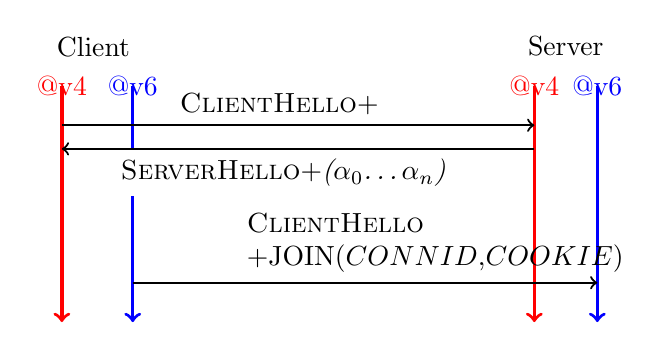
\begin{tikzpicture}
    \colorlet{lightgray}{black!20}
    \tikzstyle{arrow} = [thick,->,>=stealth]
    \tikzset{state/.style={rectangle, dashed, draw, fill=white} }
    \node[black, fill=white] at (0,10) {Client};
    \node[black, fill=white] at (6,10) {Server};
    \node[red, fill=white] at (5.6,9.5) {@v4};
    \node[blue, fill=white] at (6.4,9.5) {@v6};
    \node[red, fill=white] at (-0.4,9.5) {@v4};
    \node[blue, fill=white] at (0.5,9.5) {@v6};
    \draw[red, very thick,->] (-0.4,9.5) -- (-0.4,6.5);
    \draw[blue, very thick,->] (0.5,9.5) -- (0.5,6.5);
    \draw[red, very thick,->] (5.6,9.5) -- (5.6,6.5);
    \draw[blue, very thick,->] (6.4,9.5) -- (6.4,6.5);
   \draw[black, thick, ->] (-0.4,9) -- (5.6,9) node [midway, fill=white, above,
   text width=3cm] {\textsc{ClientHello}+\emph{\tcpls}};
   \draw[black, thick, <-] (-0.4,8.7) -- (5.6,8.7) node [midway, fill=white, below, text width=4.5cm] {\textsc{ServerHello}+\emph{\tcpls($\alpha_0$\ldots$\alpha_n$)} };
   \draw[black, thick, ->] (0.5,7) -- (6.4,7) node [midway, fill=white, above,
   text width=3cm] {\textsc{ClientHello}\\+JOIN($CONNID$,$COOKIE$)};
  \end{tikzpicture}
  \caption{\tcpls supports the attachment of additional \tcp
    connections to a \tcpls connection. Each $\alpha_i$ is encrypted with the
    handshake key.}
  \label{fig:join-example}
\end{figure}
\paragraph*{How to Join}

\tcpls securely solves this \texttt{``connection join''} problem. For example,
consider a client connecting to a dual-stack server. Fig.~\ref{fig:join-example}
depicts the \tls messages exchanged.  The client starts with a
\textsc{ClientHello}. This includes the \tcpls extension to negotiate \tcpls.
The server replies with a \textsc{ServerHello} containing several important and
encrypted control information $\alpha$. First, the server announces its IPv4 and
IPv6 addresses. Second, it associates one connection identifier.  This
identifier uniquely identifies the connection on the server. Third, the server
provides a list of cookies that enable the client to attach additional \tcp
connections to the \tcpls connection. To attach a new connection, e.g., using
the server's IPv6 address, the client opens a \tcp connection and sends a
\textsc{ClientHello} message containing the connection identifier ($CONNID$) and
one of the cookies supplied ($COOKIE$) by the server.

The Connection identifier allows the server to attach the new \tcp connection to
the right \tcpls session, assuming the received cookie is valid. The Connection
identifier and the cookie play that same role as \mptcp's token. However, the
cookie is longer, encrypted in the initial \textsc{ServerHello} message, and
one-time use (i.e., when the server receives a valid cookie, it accepts the
connection, attaches it to the right \tcpls session, and discard the cookie).
Thanks to the cookies, the server can limit the number of \tcp connections that
a client can attach to a \tcpls connection. This prevents some denial-of-service
attacks that are possible with \mptcp.

\subsection{Secure Connection Closing}



%\fr{JOIN is explained here =)}
%Figure~\ref{fig:connmigr} shows a closer look to the \tcpls handshake, and to a
%mpjoin handshake. If the server supports \tcpls, it announces its \tcpLS Encrypted
%Extensions containing the \tcpls connection id \texttt{CONNID}, the list of
%available v4 and v6 addresses from which the sever may be reached, a list of
%one-time use cookies for mpjoin handshakes and lightweight \tcp options. A mpjoin
%handshake is carried out by calling again the \texttt{tcpls\_handshake()} with
%configured handshake properties. This handshake produces a ClientHello with a
%\texttt{JOIN} extension containing information such as the RTT of this
%connection, the \texttt{CONNID} to let the server knows to which \texttt{\tcpls}
%connection bind this \tcp connection, and a \texttt{COOKIE} which acts as an
%authentication mechanism. Note that on-path attackers cannot replay cookies,
%as they are one-time use. However, they can drop the legitimate \texttt{JOIN}
%ClientHello and send the cookie to join the \tcpls's context. The server will
%never send data through a path that has not been confirmed. Confirmation happens
%with a path challenge similar to QUIC, which an on-path attacker in not
%able to answer.

%%\begin{figure}
  %%\begin{tikzpicture}
    %%\colorlet{lightgray}{black!20}
    %%\tikzstyle{arrow} = [thick,->,>=stealth]
    %%\tikzset{state/.style={rectangle, dashed, draw, fill=white} }
    %%\node[black, fill=white] at (0.5,10) {Sender};
    %%\node[black, fill=white] at (6,10) {Receiver};
    %%\node[red, fill=white] at (5.6,9.5) {@v4};
    %%\node[blue, fill=white] at (6.4,9.5) {@v6};
    %%\draw[very thick,->] (0.5,9.5) -- (0.5,0.7);
    %%\draw[red, very thick,->] (5.6,9.5) -- (5.6,0.7);
    %%\draw[blue, very thick,->] (6.4,9.5) -- (6.4,0.7);
    %\node[fill=white] at (0,9) {tcpls\_handshake()};
    %\node[fill=white] at (6,9) {tcpls\_handshake()};
   %\draw[black, thick, ->] (0.5,8) -- (5.6,8) node [midway, fill=white, above,
   %text width=3cm]
   %{Client Hello\\+ extension \tcpls};
   %\draw[black, thick, <-] (0.5,7.7) -- (5.6,7.7) node [midway, fill=white, below,
   %text width=4.5cm] { Server Hello + extension
     %\tcpls+\{CONNID\} + \{ADD\_ADDRS\} + \{COOKIES\} + \{\tcp options\}};
   %\node[fill=white, text width=3cm] at (0.5, 5.5) {Let's migrate on the received
     %v6 addr};
   %\node[fill=white, text width=3cm] at (0.5, 4.5) {tcpls\_handshake()};
   %\draw[black, thick, ->] (0.5,4) -- (6.4,4) node [midway, fill=white, above,
   %text width=3cm]
   %{Client Hello\\+JOIN(CONNID, COOKIE)};
   %\node[fill=white, align=right] at (6.8, 4)
   %{accept()};
   %\node[fill=white, align=right] at (6.1, 3.2)
   %{tcpls\_new()\\tcpls\_handshake()\\tcpls\_accept()};
   %\node[fill=white] at (6.1, 1.9) (Callback) {CB mpjoin!};
   %\node at (7.1, 1.7) (here) {};
   %\draw [->] (Callback) to[out=-80, in=-90,looseness=1.3] (here)
   %to[out=90,in=80,looseness=1.5] (Callback);
   %\node[align=right,fill=white] at (0, 2.5)
   %{tcpls\_stream\_new()\\tcpls\_streams\_attach()\\tcpls\_stream\_close(v4)\\tcpls\_send(v6)};
   %\draw[black, thick, ->] (0.5, 1.2) -- (6.4, 1.2) node [midway, above, text
   %width=3cm] {\{APPDATA\}...\{\tcpls DATA\}...\{APPDATA\}};
  %\end{tikzpicture}
  %\caption{Messages exchanged during an application-level connection migration
    %using \tcpls's API}
  %\label{fig:connmigr}
%\end{figure}


%\begin{figure}
  %\begin{tikzpicture}
    %\colorlet{lightgray}{black!20}
    %\tikzstyle{arrow} = [thick,->,>=stealth]
    %\tikzset{state/.style={rectangle, dashed, draw, fill=white} }
    %\node[black, fill=white] at (0.5,10) {Client};
    %\node[black, fill=white] at (6,10) {Server};
    %\node[red, fill=white] at (5.6,9.5) {@v4};
    %\node[blue, fill=white] at (6.4,9.5) {@v6};
    %\draw[very thick,->] (0.5,9.5) -- (0.5,-2);
    %\draw[red,very thick,->] (6,9.5) -- (6,-2);
    %\draw[blue,very thick,->] (6.2,9.5) -- (6.2,-2);
%%    \node[fill=white] at (0,9) {tcpls\_handshake()};
%%    \node[fill=white] at (6,9) {tcpls\_handshake()};
   %\draw[black, thick, ->] (0.5,8) -- (6,7.5) node [midway, fill=white, above, text width=4cm]
   %{\begin{tabular}{l}SYN\\ClientHello[\tcpls]\end{tabular}};
   %\draw[black, thick, <-] (0.5,7) -- (6,7.5) node [midway, fill=white, below, text width=6cm] {\begin{tabular}{l}SYN+ACK ServerHello[\tcpls(id=123,\\ADDRS(@v4,@v6),C=abc,\ldots)]\end{tabular}};
%%   \node[fill=white, text width=3cm] at (0.5, 4) {Let's migrate on the received
%%     v6 addr};
%%   \node[fill=white, text width=3cm] at (0.5, 3) {tcpls\_handshake()};
   %\draw[black, thick, ->] (0.5,2.5) -- (6.2,2) node [midway, fill=white, above, text width=4cm]
   %{\begin{tabular}{l}SYN,\\ClientHello[JOIN(id=123,C=abc)]\end{tabular}};
%%   \node[fill=white, align=right] at (6.8, 2.5)
%%   {accept()};
%%   \node[fill=white, align=right] at (6.1, 1.7)
%%   {tcpls\_new()\\tcpls\_handshake():};
%%   \node[fill=white] at (6.1, 0.8) (Callback) {CB mpjoin!};
%%   \node at (7.1, 0.6) (here) {};
%%   \draw [->] (Callback) to[out=-80, in=-90,looseness=1.3] (here)
%%   to[out=90,in=80,looseness=1.5] (Callback);
%   \node[fill=white] at (0, 1) {tcpls\_send(on\_v6addr);};
%   \draw[black, thick, ->] (0.5, 0) -- (6, 0) node [midway, above, text
%   width=3cm] {\{APPDATA\}...\{\tcpls DATA\}...\{APPDATA\}};
  %\end{tikzpicture}
%\end{figure}
